% Options for packages loaded elsewhere
\PassOptionsToPackage{unicode}{hyperref}
\PassOptionsToPackage{hyphens}{url}
\documentclass[
  ignorenonframetext,
]{beamer}
\newif\ifbibliography
\usepackage{pgfpages}
\setbeamertemplate{caption}[numbered]
\setbeamertemplate{caption label separator}{: }
\setbeamercolor{caption name}{fg=normal text.fg}
\beamertemplatenavigationsymbolsempty
% remove section numbering
\setbeamertemplate{part page}{
  \centering
  \begin{beamercolorbox}[sep=16pt,center]{part title}
    \usebeamerfont{part title}\insertpart\par
  \end{beamercolorbox}
}
\setbeamertemplate{section page}{
  \centering
  \begin{beamercolorbox}[sep=12pt,center]{section title}
    \usebeamerfont{section title}\insertsection\par
  \end{beamercolorbox}
}
\setbeamertemplate{subsection page}{
  \centering
  \begin{beamercolorbox}[sep=8pt,center]{subsection title}
    \usebeamerfont{subsection title}\insertsubsection\par
  \end{beamercolorbox}
}
% Prevent slide breaks in the middle of a paragraph
\widowpenalties 1 10000
\raggedbottom
\AtBeginPart{
  \frame{\partpage}
}
\AtBeginSection{
  \ifbibliography
  \else
    \frame{\sectionpage}
  \fi
}
\AtBeginSubsection{
  \frame{\subsectionpage}
}
\usepackage{iftex}
\ifPDFTeX
  \usepackage[T1]{fontenc}
  \usepackage[utf8]{inputenc}
  \usepackage{textcomp} % provide euro and other symbols
\else % if luatex or xetex
  \usepackage{unicode-math} % this also loads fontspec
  \defaultfontfeatures{Scale=MatchLowercase}
  \defaultfontfeatures[\rmfamily]{Ligatures=TeX,Scale=1}
\fi
\usepackage{lmodern}
\ifPDFTeX\else
  % xetex/luatex font selection
\fi
% Use upquote if available, for straight quotes in verbatim environments
\IfFileExists{upquote.sty}{\usepackage{upquote}}{}
\IfFileExists{microtype.sty}{% use microtype if available
  \usepackage[]{microtype}
  \UseMicrotypeSet[protrusion]{basicmath} % disable protrusion for tt fonts
}{}
\makeatletter
\@ifundefined{KOMAClassName}{% if non-KOMA class
  \IfFileExists{parskip.sty}{%
    \usepackage{parskip}
  }{% else
    \setlength{\parindent}{0pt}
    \setlength{\parskip}{6pt plus 2pt minus 1pt}}
}{% if KOMA class
  \KOMAoptions{parskip=half}}
\makeatother
\usepackage{longtable,booktabs,array}
\usepackage{caption}
\captionsetup[table]{skip=6pt}
\newcounter{none} % for unnumbered tables
\usepackage{calc} % for calculating minipage widths
\usepackage{caption}
% Make caption package work with longtable
\makeatletter
\def\fnum@table{\tablename~\thetable}
\makeatother
\usepackage{graphicx}
\makeatletter
\newsavebox\pandoc@box
\newcommand*\pandocbounded[1]{% scales image to fit in text height/width
  \sbox\pandoc@box{#1}%
  \Gscale@div\@tempa{\textheight}{\dimexpr\ht\pandoc@box+\dp\pandoc@box\relax}%
  \Gscale@div\@tempb{\linewidth}{\wd\pandoc@box}%
  \ifdim\@tempb\p@<\@tempa\p@\let\@tempa\@tempb\fi% select the smaller of both
  \ifdim\@tempa\p@<\p@\scalebox{\@tempa}{\usebox\pandoc@box}%
  \else\usebox{\pandoc@box}%
  \fi%
}
% Set default figure placement to htbp
\def\fps@figure{htbp}
\makeatother
\setlength{\emergencystretch}{3em} % prevent overfull lines
\providecommand{\tightlist}{%
  \setlength{\itemsep}{0pt}\setlength{\parskip}{0pt}}
% Auto-generated by infrastructure/rendering/_pdf_latex_helpers.py::extract_math_font_preamble.
% Minimal header passed to Pandoc via -H so Beamer slides pick up the same math font
% as the combined-PDF path. Adjust the manuscript's preamble.md to change the font globally.
\usepackage{unicode-math}
\setmathfont{latinmodern-math.otf}

% Manuscript macro/package fallbacks (newcommand -> providecommand).
% Core mathematics
\usepackage{amsmath}
\usepackage{amssymb}
% Document layout
% Tables
\usepackage{booktabs}
% Caption styling (booktabs already loaded above). Small caption font with a
% bold label ("Figure 1", "Table 2") gives the math/figure-heavy layout a
% consistent, journal-like caption rhythm without fighting pandoc-crossref —
% pandoc emits standard \caption{}, and caption/captionsetup only restyle it.
% ── Theorem environments ─────────────────────────────────────────────────
% amsthm is loaded above. The FedGVI<->Friston bridge is stated as a small
% number of theorems/definitions/lemmas/propositions/corollaries; sharing one
% counter (definition/lemma/proposition/corollary all step the `theorem`
% counter) gives a single monotone numbering 1, 2, 3, ... across all kinds, so
% authors can reference them as Theorem 1, Definition 2, Corollary 3 without a
% per-kind counter drifting out of order. Plain style for theorem-like results,
% definition style (upright body) for definitions.
% (algorithm2e intentionally not loaded: this manuscript states results as
% numbered amsthm Theorems/Definitions, not algorithm2e pseudocode.)
% Code listings
\usepackage{listings}
% Typography and formatting
% (siunitx intentionally not loaded: no \SI/\num units appear in this manuscript.)
% Cross-references and citations
% (cleveref and titlesec intentionally not loaded: unavailable in this TeX tree
% and not required. Cross-references resolve through pandoc-crossref's own
% \ref-style names — no \cref appears — and section heading styling falls back
% to the pandoc/LaTeX defaults.)
% ── TeX Live Basic-compatible mono font for code listings ────────────
% Latin Modern Mono is bundled with TeX Live Basic and keeps the manuscript
% renderable on minimal TeX installations. Mathematical Unicode coverage is
% provided separately by Latin Modern Math below, so the code font does not
% need a private JuliaMono installation.
%
% Use the TeX font filename rather than the system-family name: the minimal
% TeX Live fontconfig database may not register the OpenType family even though
% kpsewhich can resolve the bundled files.
% Math font for unicode-math: Latin Modern Math (TeX Live) has full BMP
% coverage including U+2223 (\mid), U+226A/226B (\ll/\gg), and the Greek/
% blackboard letters used in equations. Without an explicit \setmathfont,
% unicode-math falls back to lmroman text font which lacks several glyphs
% and emits "Missing character" warnings on every \mid in math mode.

% Slide layout defaults for warning-clean scientific decks.
\usepackage{etoolbox}
\IfFileExists{xurl.sty}{\usepackage{xurl}}{}
\IfFileExists{seqsplit.sty}{\usepackage{seqsplit}}{\newcommand{\seqsplit}[1]{#1}}
\protected\def\breakseq#1{\seqsplit{#1}}
\protected\def\breaktt#1{\begingroup\ttfamily\seqsplit{#1}\endgroup}
\setlength{\emergencystretch}{6em}
\tolerance=5000
\hbadness=10000
\hfuzz=1pt
\setlength{\tabcolsep}{2pt}
\AtBeginEnvironment{longtable}{\tiny\renewcommand{\arraystretch}{0.86}\setlength{\tabcolsep}{1pt}}
\AtBeginEnvironment{tabular}{\tiny\renewcommand{\arraystretch}{0.86}\setlength{\tabcolsep}{1pt}}
\AtBeginEnvironment{equation}{\tiny}
\AtBeginEnvironment{equation*}{\tiny}
\AtBeginEnvironment{align}{\tiny}
\AtBeginEnvironment{align*}{\tiny}
\AtBeginEnvironment{itemize}{\footnotesize}
\AtBeginEnvironment{enumerate}{\footnotesize}
\AtBeginEnvironment{description}{\footnotesize}
\setbeamerfont{caption}{size=\tiny}
\setbeamerfont{caption name}{size=\tiny}
\setbeamerfont{normal text}{size=\small}
\setbeamerfont{frametitle}{size=\small}
\setbeamerfont{section title}{size=\footnotesize}
\setbeamerfont{subsection title}{size=\footnotesize}
\setbeamertemplate{section page}{%
  \centering
  \begin{beamercolorbox}[sep=12pt,center,wd=\paperwidth]{section title}
    \parbox{0.86\paperwidth}{\centering\usebeamerfont{section title}\insertsection\par}
  \end{beamercolorbox}
}
\setbeamertemplate{subsection page}{%
  \centering
  \begin{beamercolorbox}[sep=8pt,center,wd=\paperwidth]{subsection title}
    \parbox{0.86\paperwidth}{\centering\usebeamerfont{subsection title}\insertsubsection\par}
  \end{beamercolorbox}
}
\setlength{\abovecaptionskip}{2pt}
\setlength{\belowcaptionskip}{0pt}

% Natbib and cross-reference fallbacks — slides don't load natbib
% or cleveref, but combined-PDF manuscript prose may emit these
% commands. The fallback renders citations as a bracketed key list
% and cross-references as detokenized labels so slides don't fail on
% undefined control sequences or raw underscores. \providecommand is
% a no-op if packages load later.
\providecommand{\citep}[1]{[#1]}
\providecommand{\citet}[1]{#1}
\providecommand{\citealp}[1]{#1}
\providecommand{\citeauthor}[1]{#1}
\providecommand{\citeyear}[1]{#1}
\providecommand{\cref}[1]{\texttt{\detokenize{#1}}}
\providecommand{\Cref}[1]{\texttt{\detokenize{#1}}}
\providecommand{\crefrange}[2]{\texttt{\detokenize{#1}}--\texttt{\detokenize{#2}}}
\providecommand{\Crefrange}[2]{\texttt{\detokenize{#1}}--\texttt{\detokenize{#2}}}
\providecommand{\paragraph}[1]{\textbf{#1}\ }

\newtheorem{proposition}{Proposition}
\newtheorem{hypothesis}{Hypothesis}
\newtheorem{remark}[theorem]{Remark}
\newtheorem{axiom}{Axiom}
\newtheorem{property}{Property}
\usepackage{bookmark}
\IfFileExists{xurl.sty}{\usepackage{xurl}}{} % add URL line breaks if available
\urlstyle{same}
% fallback for those not using the hyperref driver hyperxmp:
\makeatletter
\@ifundefined{xmpquote}{\newcommand{\xmpquote}[1]{#1}}{}
\makeatother
\hypersetup{
  hidelinks,
  pdfcreator={LaTeX via pandoc}}

\author{\texorpdfstring{}{}}
\date{}

\begin{document}

\begin{frame}[fragile,allowframebreaks]{Structure learning: does the
hierarchy earn its depth?}
\protect\phantomsection\label{sec:results-hierarchical-bmr}
Study 7 shows the 3-level agent runs and federates end to end, but a
deeper model is only warranted if the extra level carries information.
We close the loop with a structure-learning test: given a trained
hierarchy and one leaf observation, does Bayesian model reduction
correctly decide whether the top meta-context level should be
\emph{kept} or \emph{pruned}?

We reduce at the level granularity
(:func:\breaktt{fedference.bayesian\_model\_reduction.hierarchical\_reduce}).
For each non-leaf level we measure its \textbf{Bayesian surprise}
\(\mathrm{KL}(q_i \,\|\, \tilde p_i)\) --- how far the leaf observation
moves that level's belief \(q_i\) from its top-down prior
\(\tilde p_i\). A level whose belief the data never move carries no
structure and is prunable; an informative level moves and is kept. This
is an inference-derived divergence, not a model re-fit, so it cannot
\end{frame}

\begin{frame}[fragile,allowframebreaks]{Structure learning: does the
hierarchy earn its depth?}
manufacture a difference the generative model does not contain.

The test is directional by construction. We build two 3-level worlds
that differ \emph{only} in the top level's conditioned priors: a
\textbf{degenerate} world whose meta-context is non-gating (both
meta-context states predict the same context distribution) and an
\textbf{informative} world whose meta-context sharply distinguishes the
two contexts. On the degenerate world the top level earns a Bayesian
surprise of 0.000 nats and is flagged prunable (recovers the two-level
structure: Yes); on the informative world the same level earns 0.328
nats and is kept (Yes); fig.~\ref{fig:hierarchical-bmr} shows the
per-level surprise for both worlds side by side. Because the two worlds
share every other parameter, the opposite verdict is attributable to the
meta-context's information alone --- the reduction discovers the right
depth rather than assuming it.
\end{frame}

\begin{frame}[fragile,allowframebreaks]{Structure learning: does the
hierarchy earn its depth?}

\begin{figure}
\centering
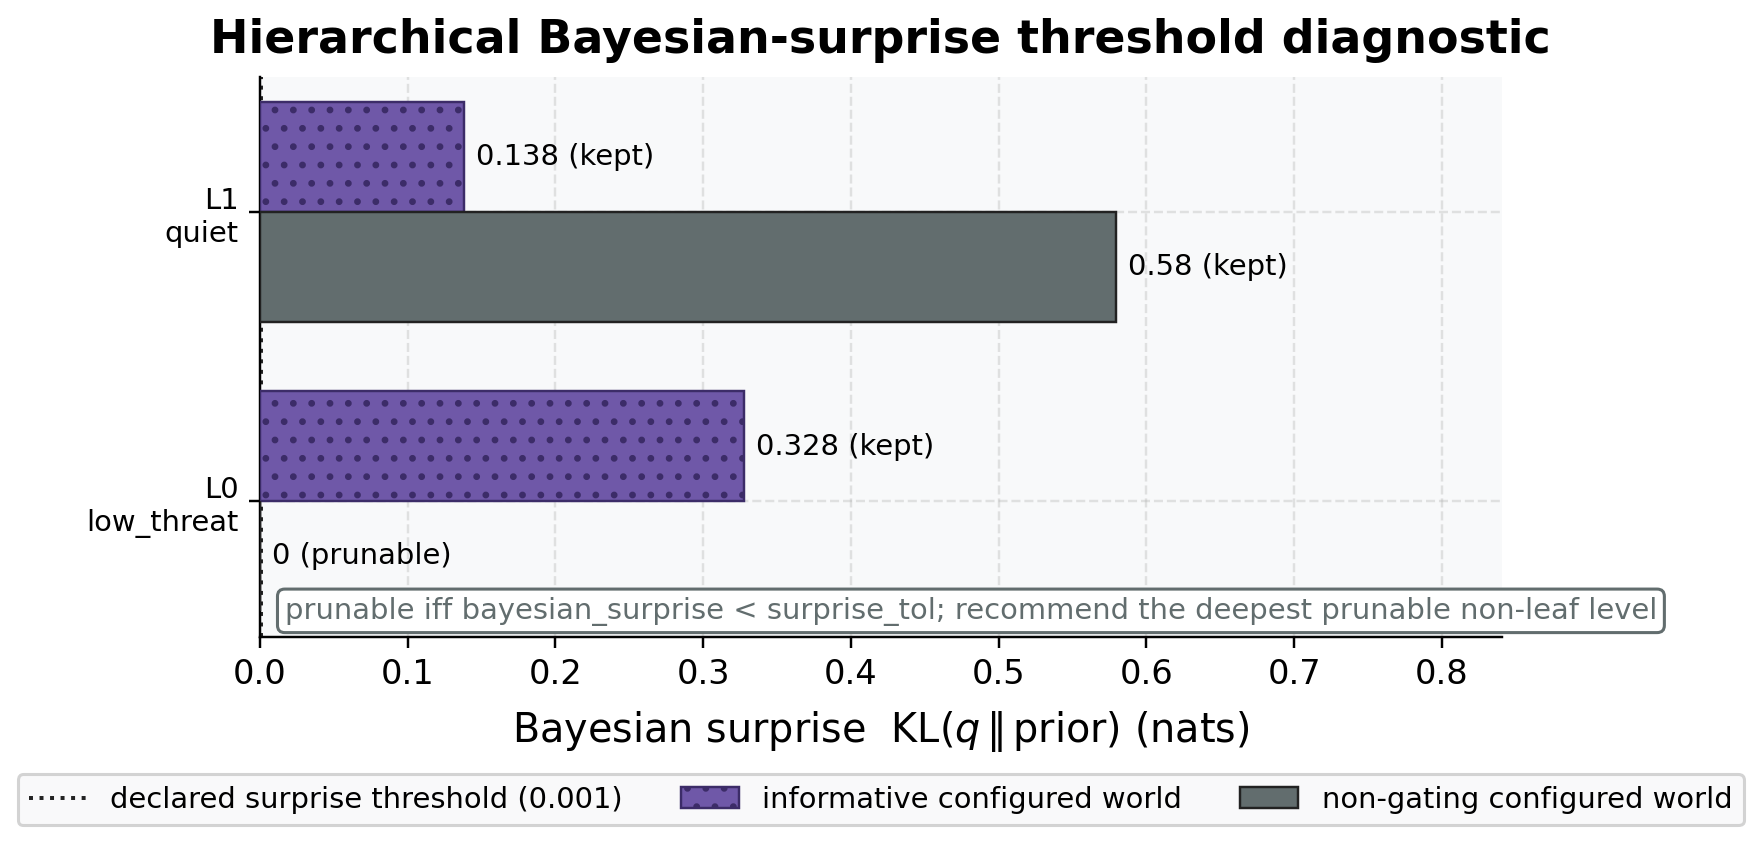
\includegraphics[width=0.8\linewidth,height=0.40\textheight,keepaspectratio,alt={Per-level Bayesian surprise and prune/keep decisions for two hierarchical worlds. Source relation: original project BMR structure-learning diagnostic related to the mechanism in Friston et al.~Fig. 9; estimand: per-level Bayesian surprise in nats and the resulting prune/keep decision; uncertainty: deterministic schematic worlds, so no resampling interval is shown. Per-level Bayesian surprise for the two 3-level worlds. y-axis: the non-leaf reduction targets, indexed top-down from the reduction routine as level 0 = the meta-context (the topmost non-leaf level, L3 in the location-first L1/L2/L3 convention used elsewhere) and level 1 = the context (L2); the leaf location level (L1) is never a reduction target. x-axis: Bayesian surprise \textbackslash mathrm\{KL\}(q \textbackslash,\textbackslash\textbar\textbackslash, \textbackslash text\{prior\}) in nats --- the information the leaf observation added at that level. Blue bars: the informative world (top level kept). Grey bars: the degenerate world (top level prunable). The dashed red line is the prune threshold; a level whose surprise falls below it is structurally unnecessary. The degenerate meta-context (grey, level 0) sits at 0.000 nats and is pruned, recovering the two-level model, while the informative meta-context (blue, level 0) at 0.328 nats is retained; both worlds keep the context level (level 1). Deterministic schematic worlds (no resampling), so no error band is applicable.}]{../figures/hierarchical_bmr.png}
\caption{Per-level Bayesian surprise and prune/keep decisions for two
hierarchical worlds. Source relation: original project BMR
structure-learning diagnostic related to the mechanism in Friston et
al.~Fig. 9; estimand: per-level Bayesian surprise in nats and the
resulting prune/keep decision; uncertainty: deterministic schematic
worlds, so no resampling interval is shown. Per-level Bayesian surprise
for the two 3-level worlds. y-axis: the non-leaf reduction targets,
indexed top-down from the reduction routine as level 0 = the
meta-context (the topmost non-leaf level, L3 in the location-first
L1/L2/L3 convention used elsewhere) and level 1 = the context (L2); the
leaf location level (L1) is never a reduction target. x-axis: Bayesian
surprise \(\mathrm{KL}(q \,\|\, \text{prior})\) in nats --- the
information the leaf observation added at that level. Blue bars: the
informative world (top level kept). Grey bars: the degenerate world (top
level prunable). The dashed red line is the prune threshold; a level
whose surprise falls below it is structurally unnecessary. The
degenerate meta-context (grey, level 0) sits at 0.000 nats and is
pruned, recovering the two-level model, while the informative
meta-context (blue, level 0) at 0.328 nats is retained; both worlds keep
the context level (level 1). Deterministic schematic worlds (no
resampling), so no error band is
applicable.}\label{fig:hierarchical-bmr}
\end{figure}

\end{frame}

\begin{frame}[fragile,allowframebreaks]{Structure learning: does the
hierarchy earn its depth?}
This is the same Beta-function model-reduction machinery that drives the
emergence study (sec.~7.4,
eq.~16), lifted from pruning redundant \emph{states}
within one level to pruning a redundant \emph{level} of the hierarchy
--- an honest, tested answer to ``how deep should the generative model
be?'' that the data, not the modeler, decides.
\end{frame}

\end{document}
